\chapter{Quantum Dots}

\section{One Dimension}

We blast the guy with 
\begin{equation}
    E(t) = E_0\sin^2\left(\frac{t\pi}{T}\right)\cos(\omega t),
\end{equation}
which defines a laser pulse, consisting of several parts. Blah blah blah.

\begin{figure}
    \centering
    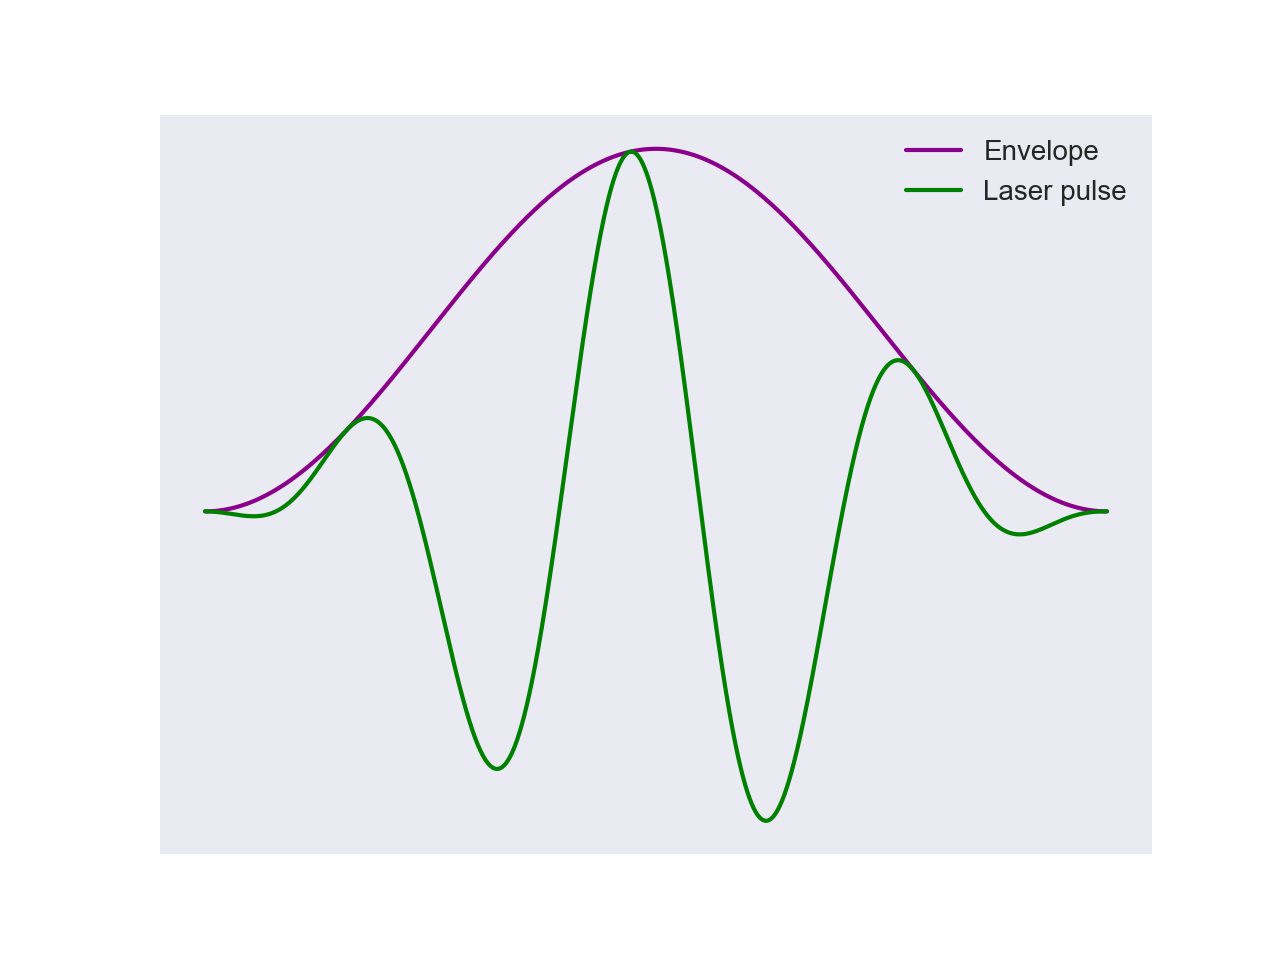
\includegraphics[width=0.6\textwidth]{results/figures/heaviside_laser.png} 
    \caption{}
    \label{fig:heaviside_laser}
\end{figure}

\begin{figure}
    \centering
    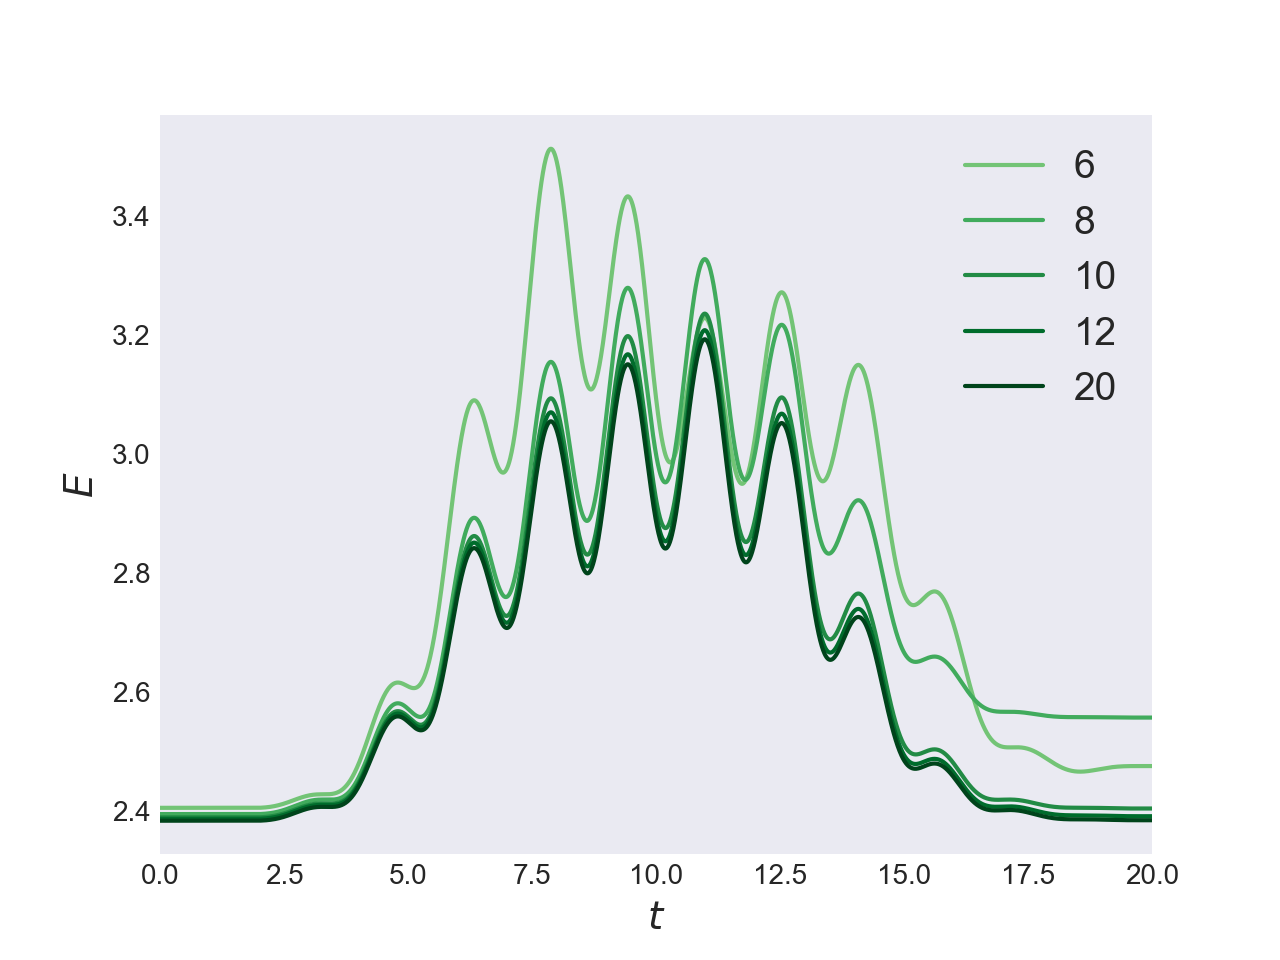
\includegraphics[width=0.9\textwidth]{results/figures/1D/n=2energy.png} 
    \caption{Energy $n=2$.}
    \label{fig:1d_n2_E}
\end{figure}

\begin{figure}
    \centering
    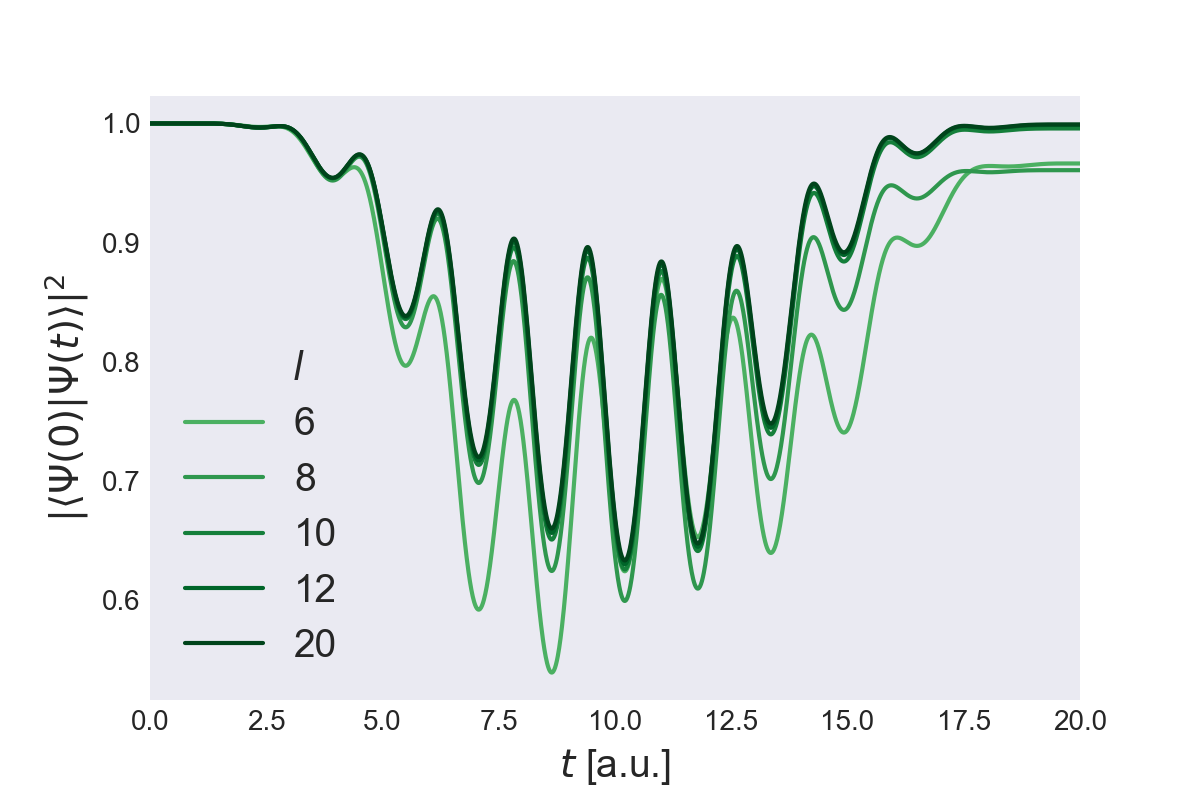
\includegraphics[width=0.9\textwidth]{results/figures/1D/n=2overlap.png} 
    \caption{}
    \label{}
\end{figure}